\documentclass[12pt,a4paper]{article}

% ─── Encodage & Langue ───────────────────────────────────────────
\usepackage[utf8]{inputenc}
\usepackage[T1]{fontenc}
\usepackage[french]{babel}

% ─── Mise en page ────────────────────────────────────────────────
\usepackage[margin=2.5cm]{geometry}
\usepackage{setspace}
\onehalfspacing

% ─── Typographie ─────────────────────────────────────────────────
\usepackage{lmodern}
\usepackage{microtype}

% ─── Figures & Tableaux ──────────────────────────────────────────
\usepackage{graphicx}
\usepackage{float}
\usepackage{booktabs}
\usepackage{array}
\usepackage{caption}
\usepackage{subcaption}

% ─── Maths ───────────────────────────────────────────────────────
\usepackage{amsmath}
\usepackage{amssymb}

% ─── Code & Verbatim ─────────────────────────────────────────────
\usepackage{listings}
\usepackage{xcolor}
\lstset{
  basicstyle=\ttfamily\small,
  breaklines=true,
  frame=single,
  backgroundcolor=\color{gray!10},
  commentstyle=\color{gray},
  keywordstyle=\color{blue},
}

% ─── Hyperliens ──────────────────────────────────────────────────
\usepackage[hidelinks]{hyperref}

% ─── Bibliographie ───────────────────────────────────────────────
\usepackage{natbib}
\bibliographystyle{plainnat}

% ─────────────────────────────────────────────────────────────────
\title{\textbf{Few-Shot Learning pour l'Inférence en Langue Naturelle en Français}\\[0.5em]
{\large Évaluation de LLMs génératifs par l'approche Label-Only}\\[1em]
{\normalsize TER M1 -- Rapport d'expériences}}

\author{Reda Ammari}
\date{Mai 2026}

\begin{document}

\maketitle
\tableofcontents
\newpage

% ─────────────────────────────────────────────────────────────────
\section{Expériences : Few-Shot Label-Only sur LLMs génératifs}

\subsection{Protocole expérimental}

\subsubsection{Technique utilisée : Label-Only Few-Shot}

L'approche retenue dans ce travail est le \textbf{Few-Shot Label-Only}, une variante du prompting en contexte (\textit{in-context learning}) appliquée à la tâche d'Inférence en Langue Naturelle (NLI). Contrairement au \textit{Chain-of-Thought} qui demande au modèle de produire un raisonnement explicite, le mode Label-Only contraint le modèle à répondre \emph{uniquement} avec le label prédit, sans justification intermédiaire.

Le prompt suit la structure suivante :

\begin{enumerate}
    \item Un \textbf{message système} définit la tâche et l'espace des labels possibles (\texttt{entailment}, \texttt{neutral}, \texttt{contradiction} pour les datasets 3 classes ; \texttt{non-contradiction}, \texttt{contradiction} pour les datasets binaires).
    \item Entre $0$ et $10$ \textbf{exemples annotés} (les \textit{shots}), sélectionnés de façon équilibrée par classe depuis le dataset d'entraînement avec une graine aléatoire fixée.
    \item L'\textbf{exemple de test} à classer, présenté sans label.
\end{enumerate}

\begin{verbatim}
[Système] Tu es un expert en NLI en français. 
Les labels possibles sont : entailment, neutral, contradiction.
Réponds UNIQUEMENT avec le label exact, rien d'autre.

[User] Voici 3 exemple(s) :
Prémisse : Le chat dort sur le canapé.
Hypothèse : Un animal est allongé sur un meuble.
Label : entailment
---
[...autres exemples...]
---
Maintenant, classe cet exemple :
Prémisse : ...
Hypothèse : ...
Label :
\end{verbatim}

Cette formulation présente deux avantages majeurs : (1) elle supprime tout bruit lié à la variabilité du raisonnement généré et (2) elle facilite l'extraction automatique des prédictions via une simple correspondance de chaîne de caractères. Le \textbf{parse rate} mesure la proportion de réponses correctement parsées ; un parse rate de 100\% indique que le modèle a strictement respecté le format attendu.

\subsubsection{Modèles évalués}

Six grands modèles de langue génératifs ont été évalués, tous chargés en quantification 4-bit (NF4) via \texttt{BitsAndBytes} pour tenir dans la mémoire GPU disponible sur Kaggle (T4 $\times$2 ou P100). Le Tableau~\ref{tab:models} récapitule leurs caractéristiques.

\begin{table}[h]
\centering
\caption{Modèles LLMs évalués dans les expériences Few-Shot Label-Only.}
\label{tab:models}
\begin{tabular}{lrll}
\toprule
\textbf{Modèle} & \textbf{Params} & \textbf{Identifiant HuggingFace} & \textbf{Architecture} \\
\midrule
Phi-3 Mini       & 3.8B  & \texttt{microsoft/Phi-3-mini-4k-instruct}          & Transformer dense \\
Mistral 7B       & 7B    & \texttt{mistralai/Mistral-7B-Instruct-v0.3}        & Transformer dense \\
Qwen 2.5 7B      & 7B    & \texttt{Qwen/Qwen2.5-7B-Instruct}                  & Transformer dense \\
Llama 3 8B       & 8B    & \texttt{meta-llama/Llama-3.1-8B-Instruct}          & Transformer dense \\
Gemma 2 9B       & 9B    & \texttt{google/gemma-2-9b-it}                      & Transformer dense \\
DeepSeek R1 Dist.& 8B    & \texttt{deepseek-ai/DeepSeek-R1-Distill-Llama-8B}  & Distillation RL \\
\bottomrule
\end{tabular}
\end{table}

\subsubsection{Datasets utilisés}

Cinq corpus NLI en français ont été mobilisés (Tableau~\ref{tab:datasets}). Pour chaque configuration expérimentale, un dataset joue le rôle de \textbf{source de few-shot} (exemples annotés fournis dans le prompt) et un autre joue le rôle d'\textbf{ensemble d'évaluation} (exemples non vus par le modèle). Cette distinction est fondamentale : le modèle ne voit \emph{jamais} les labels du dataset d'évaluation, uniquement ceux des exemples few-shot.

\begin{table}[h]
\centering
\caption{Datasets NLI français utilisés dans les expériences.}
\label{tab:datasets}
\begin{tabular}{llcc}
\toprule
\textbf{Dataset} & \textbf{Description} & \textbf{Classes} & \textbf{Rôle} \\
\midrule
FraCaS-GQ  & Corpus de raisonnement logique (générique) & 3 & Train / Éval \\
GQNLI      & Questions générales NLI en français         & 3 & Train / Éval \\
RTE3       & Reconnaissance de l'implication textuelle   & 2 & Train / Éval \\
SICK-FR    & Compréhension de l'inférence et compositionalité & 3 & Train / Éval \\
DACCORD    & Corpus de dialogue et contradiction         & 2 & Train uniquement \\
\bottomrule
\end{tabular}
\end{table}

\paragraph{Protocole d'évaluation.}
Pour chaque combinaison (dataset\_train, dataset\_eval, n\_shots, seed), jusqu'à 300 exemples équilibrés par classe sont tirés du dataset d'évaluation. Les few-shot examples sont tirés \emph{indépendamment} depuis le dataset d'entraînement, avec une sélection équilibrée par classe. Trois graines aléatoires sont utilisées (42, 123, 999) pour estimer la variance des résultats. Il n'y a \textbf{pas d'entraînement ni de fine-tuning} : le modèle est utilisé en inférence pure.

\subsubsection{Nombre de shots et configurations}

Les valeurs de $k$ (nombre d'exemples few-shot) testées sont : $k \in \{0, 1, 3, 5, 10\}$, couvrant ainsi le spectre du \textit{zero-shot} (aucun exemple) au \textit{10-shot}. Au total, le sweep complet représente :

\[
5 \text{ datasets\_train} \times 4 \text{ datasets\_eval} \times 5 \text{ shots} \times 3 \text{ seeds} = 300 \text{ runs par modèle}
\]

\subsection{Résultats globaux}

\subsubsection{Classement général des modèles}

Le Tableau~\ref{tab:ranking} présente l'accuracy moyenne sur toutes les combinaisons (datasets, shots, seeds) pour chaque modèle.

\begin{table}[h]
\centering
\caption{Classement global des LLMs — accuracy moyenne (toutes configurations).}
\label{tab:ranking}
\begin{tabular}{lrccr}
\toprule
\textbf{Modèle} & \textbf{Params} & \textbf{Accuracy moy.} & \textbf{F1 macro moy.} & \textbf{Nb runs} \\
\midrule
Gemma 2 9B   & 9B  & \textbf{71.4\%} & 0.640 & 40  \\
Qwen 2.5 7B  & 7B  & 68.3\%          & 0.680 & 278 \\
Mistral 7B   & 7B  & 64.1\%          & 0.615 & 61  \\
Llama 3 8B   & 8B  & 60.3\%          & 0.534 & 261 \\
Phi-3 3.8B   & 3.8B& 56.9\%          & 0.533 & 229 \\
\bottomrule
\end{tabular}
\end{table}

\textbf{Gemma 2 9B} obtient le meilleur score (71.4\%), suivi de \textbf{Qwen 2.5 7B} (68.3\%). Fait notable : Qwen 2.5 7B surpasse Mistral 7B de 4 points d'accuracy malgré un nombre de paramètres identique, ce qui indique que la qualité de l'entraînement du modèle et son alignement multilingue jouent un rôle déterminant, au-delà de la seule taille.

\subsubsection{Effet du nombre de shots}

La Figure~\ref{fig:shots} illustre l'évolution de l'accuracy en fonction du nombre de shots pour chaque modèle.

\begin{figure}[h]
\centering
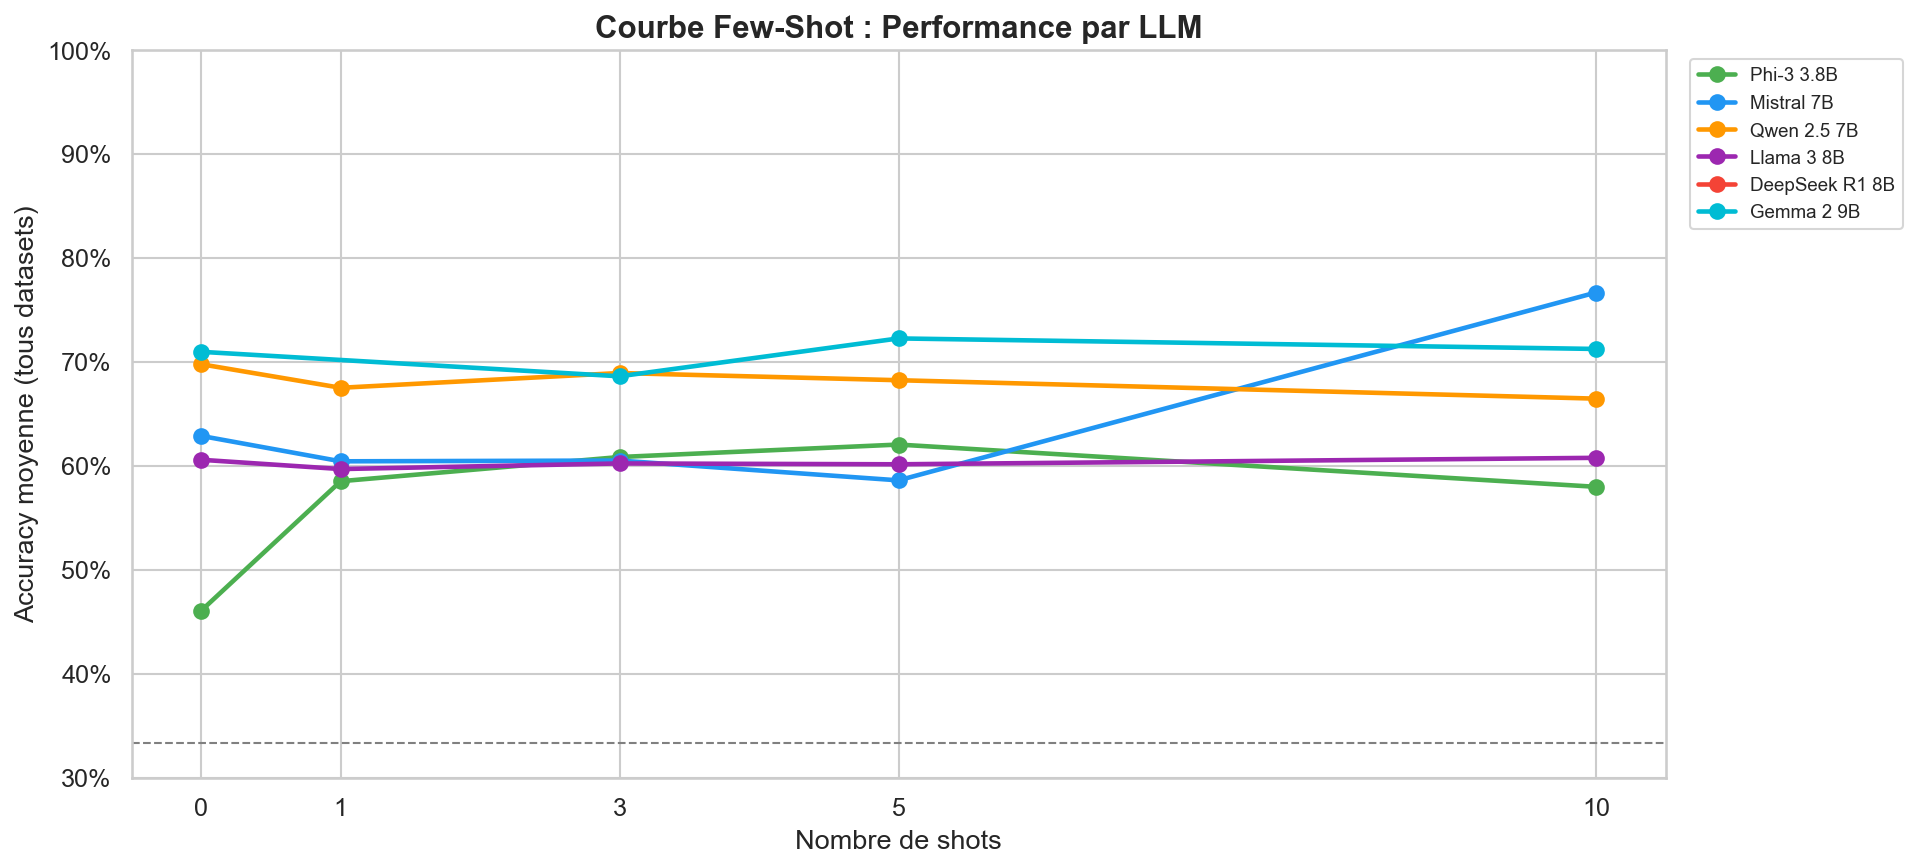
\includegraphics[width=\textwidth]{../results/label_only_plots/fig1_accuracy_vs_shots.png}
\caption{Accuracy moyenne en fonction du nombre de shots few-shot, par modèle LLM.}
\label{fig:shots}
\end{figure}

Plusieurs observations se dégagent :

\begin{itemize}
    \item \textbf{Gemma 2 9B} présente des performances stables et élevées dès le zero-shot (71.0\%), avec un léger pic à 5 shots (72.3\%). Cela suggère que ce modèle possède déjà une connaissance implicite de la tâche NLI sans exemples supplémentaires.
    \item \textbf{Qwen 2.5 7B} montre un profil similaire : de bonnes performances zero-shot (69.8\%) qui restent stables avec les shots. Le modèle semble peu sensible aux exemples en contexte.
    \item \textbf{Phi-3 3.8B} bénéficie le plus clairement du few-shot : son accuracy passe de 46.1\% en zero-shot à 62.1\% en 5-shot, soit un gain de \textbf{+16 points}. Ce phénomène est caractéristique des petits modèles qui ont besoin d'exemples pour comprendre le format de la tâche.
    \item \textbf{Mistral 7B} montre un comportement atypique avec un pic à 10 shots (76.7\%), supérieur à ses performances sur les autres configurations. Cela peut s'expliquer par une meilleure utilisation des exemples lorsqu'ils sont nombreux et diversifiés.
    \item \textbf{Llama 3 8B} présente des performances relativement stables mais basses (60--61\%) sur toutes les configurations de shots, suggérant une certaine limitation inhérente au modèle pour cette tâche en français.
\end{itemize}

\subsubsection{Effet de la taille du modèle}

\begin{figure}[h]
\centering
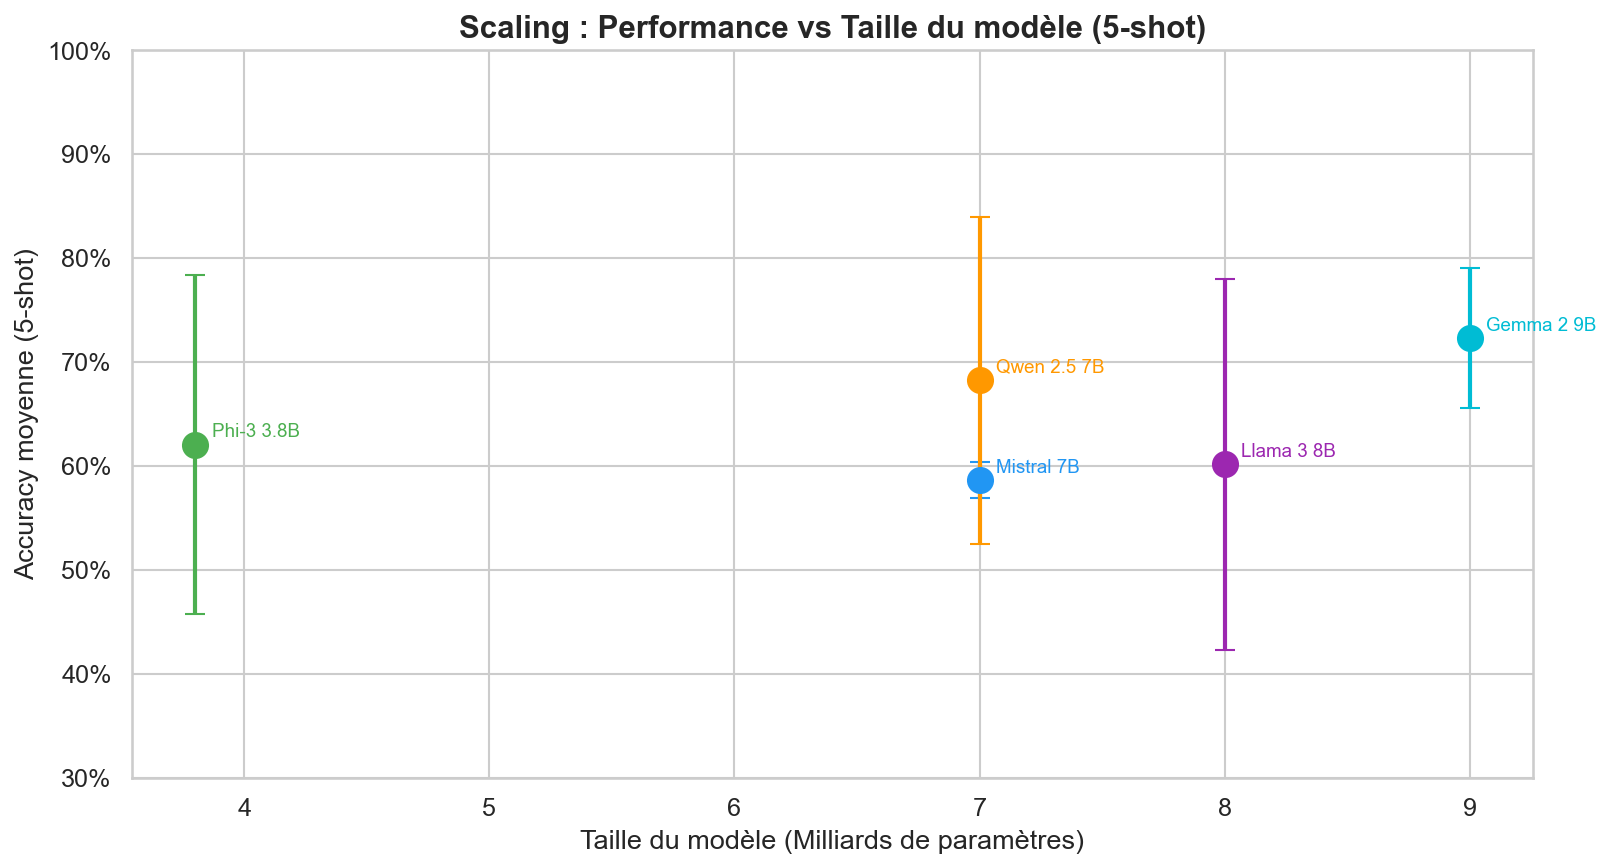
\includegraphics[width=0.85\textwidth]{../results/label_only_plots/fig2_accuracy_vs_params.png}
\caption{Accuracy moyenne (5-shot) en fonction du nombre de paramètres du modèle.}
\label{fig:params}
\end{figure}

La Figure~\ref{fig:params} montre la relation entre la taille du modèle et sa performance en configuration 5-shot. Contrairement à ce que la loi de scaling prédirait naïvement, la relation n'est pas strictement monotone :

\begin{itemize}
    \item Phi-3 3.8B ($\approx$62\%) $<$ Llama 3 8B ($\approx$60\%) $<$ Mistral 7B ($\approx$59\%) $<$ Qwen 2.5 7B ($\approx$68\%) $<$ Gemma 2 9B ($\approx$72\%)
\end{itemize}

La taille est corrélée positivement avec la performance, mais les \textbf{données d'entraînement et l'alignement multilingue} semblent dominer. Qwen 2.5 7B et Gemma 2 9B, tous deux entraînés sur des corpus massifs multilingues incluant le français, surpassent significativement des modèles plus axés sur l'anglais comme Llama 3 8B.

\subsection{Analyse cross-dataset}

\subsubsection{Généralisation : Intra vs Cross-dataset}

\begin{figure}[h]
\centering
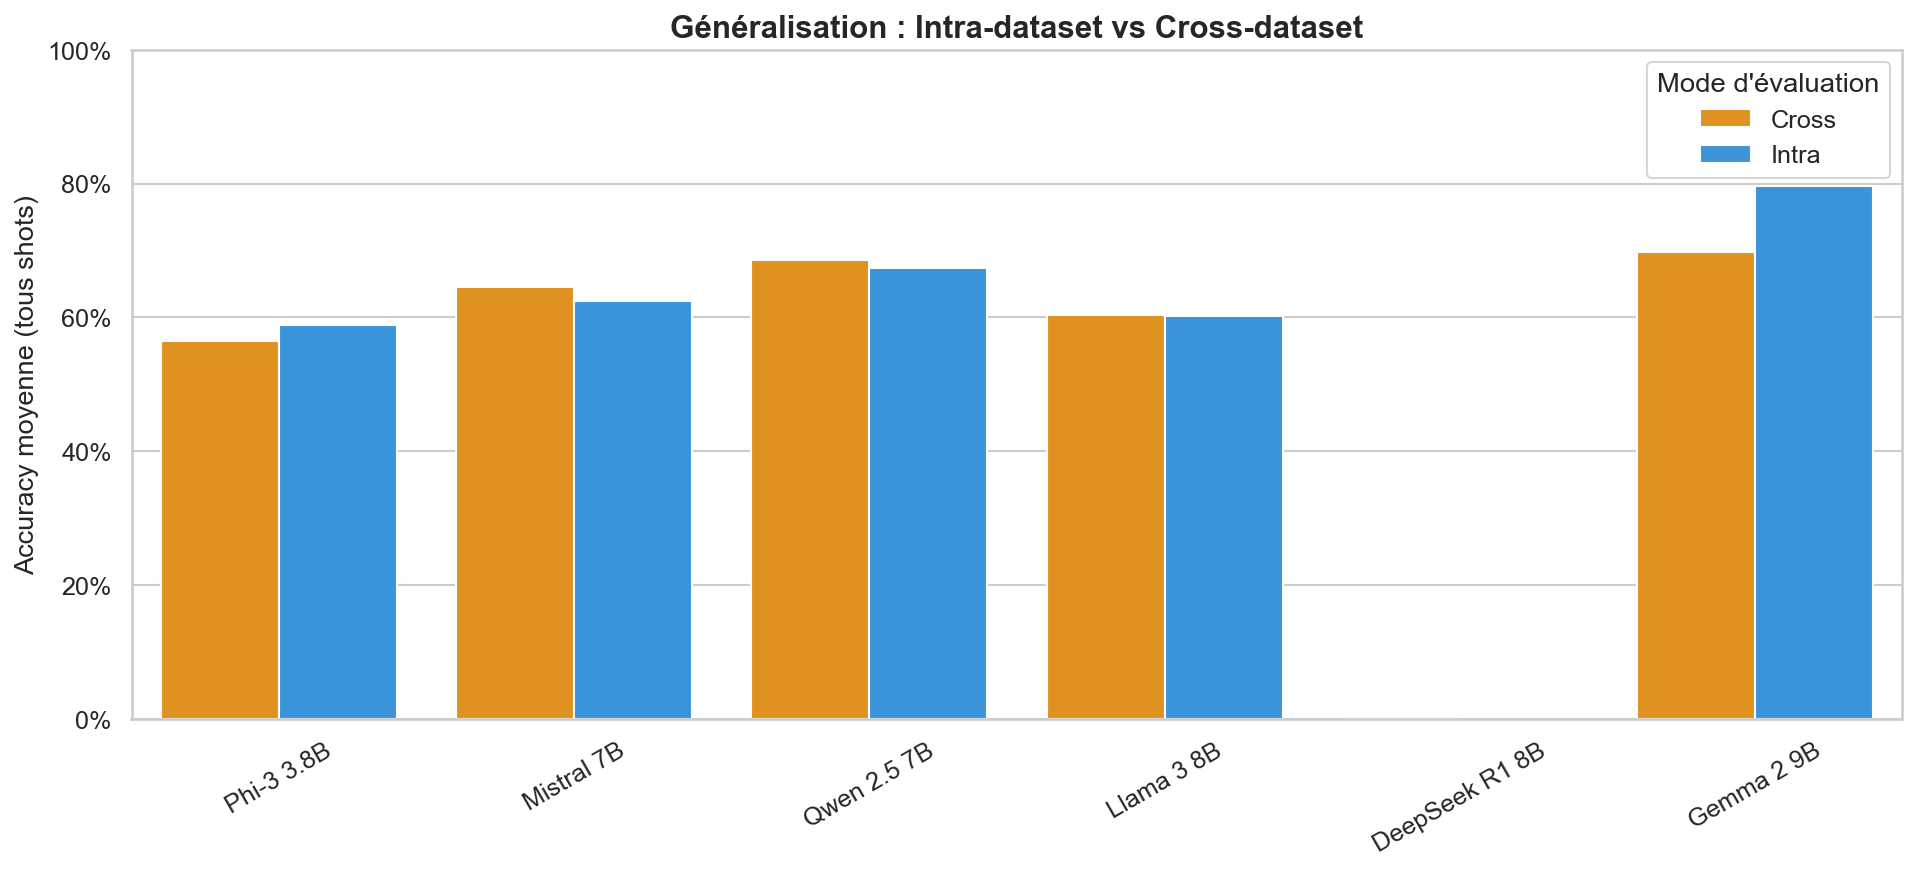
\includegraphics[width=\textwidth]{../results/label_only_plots/fig3_intra_vs_cross.png}
\caption{Comparaison des performances intra-dataset (train = eval) vs cross-dataset (train $\neq$ eval).}
\label{fig:intracross}
\end{figure}

La Figure~\ref{fig:intracross} révèle un phénomène important : pour la plupart des modèles, la performance en mode intra-dataset est légèrement supérieure ou similaire au mode cross-dataset. Ce résultat est attendu : les exemples few-shot issus du même domaine que l'évaluation sont naturellement plus pertinents pour guider le modèle.

Cependant, l'écart reste \textbf{modeste} (typiquement $< 5$ points d'accuracy), ce qui démontre une bonne capacité de généralisation des LLMs évalués. Gemma 2 montre l'écart le plus net : 79.6\% en intra contre 69.7\% en cross, soit \textbf{-9.9 points}, suggérant qu'il profite davantage de l'homogénéité des exemples.

\subsubsection{Heatmaps cross-dataset}

\begin{figure}[h]
\centering
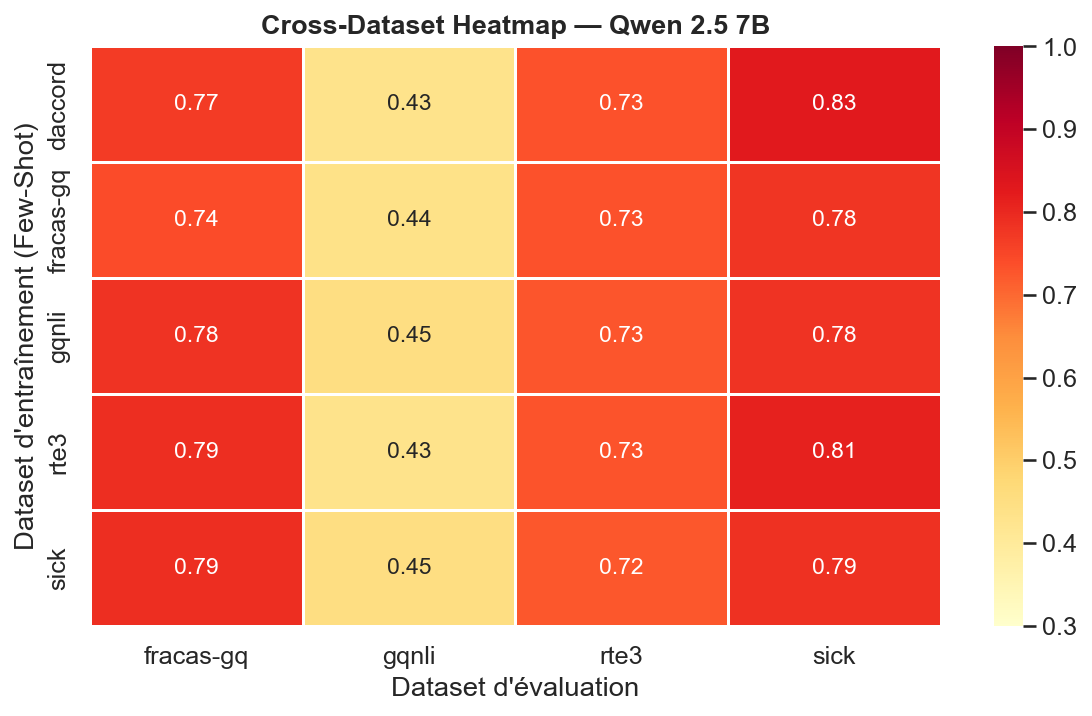
\includegraphics[width=0.48\textwidth]{../results/label_only_plots/fig4_heatmap_qwen_25_7b.png}
\hfill
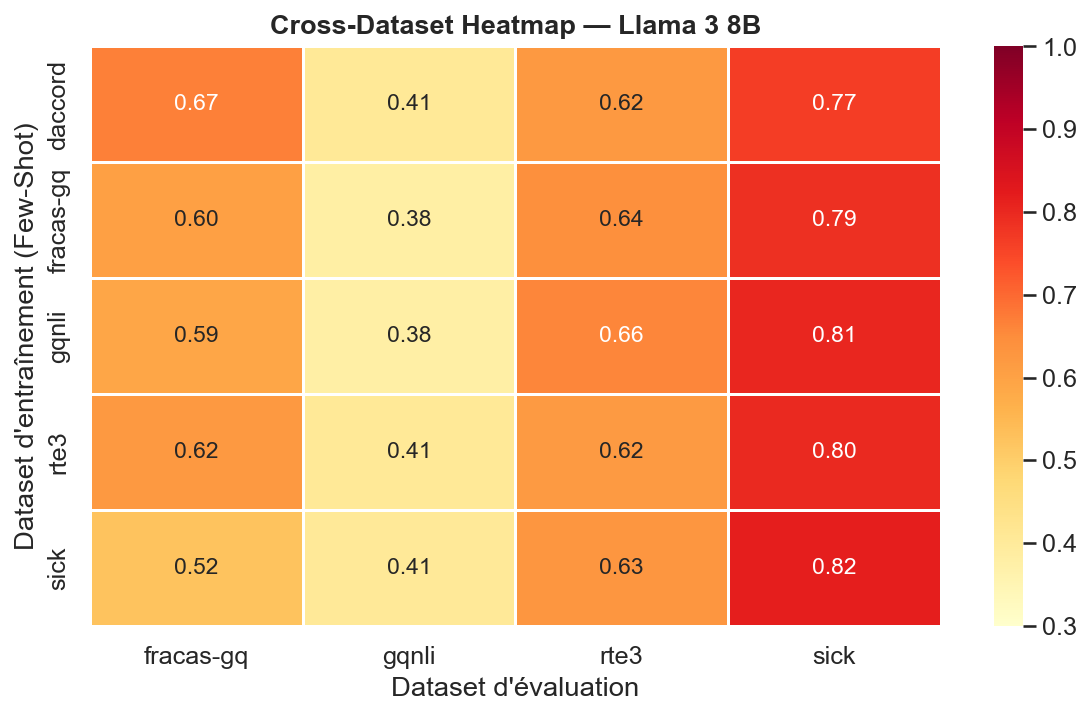
\includegraphics[width=0.48\textwidth]{../results/label_only_plots/fig4_heatmap_llama_3_8b.png}
\caption{Heatmaps cross-dataset : accuracy moyenne par combinaison (train, eval) pour Qwen 2.5 7B (gauche) et Llama 3 8B (droite).}
\label{fig:heatmaps}
\end{figure}

Les heatmaps (Figure~\ref{fig:heatmaps}) révèlent des patterns importants :

\begin{itemize}
    \item Le dataset \textbf{SICK} en évaluation obtient systématiquement les meilleures performances (jusqu'à 79.8\% pour Qwen). SICK contient des paires prémisse/hypothèse très clairement séparables sémantiquement, ce qui facilite la tâche.
    \item Le dataset \textbf{GQNLI} en évaluation donne les scores les plus bas (40--44\% selon le modèle), proche de la chance pour 3 classes. Ce corpus, centré sur des questions générales ouvertes, représente le transfert le plus difficile.
    \item \textbf{FraCaS-GQ} montre une variance élevée selon la source des exemples (de 53\% à 77\% selon le modèle), reflétant la nature logique et formelle de ce corpus.
\end{itemize}

\subsubsection{Performance par dataset d'évaluation}

\begin{figure}[h]
\centering
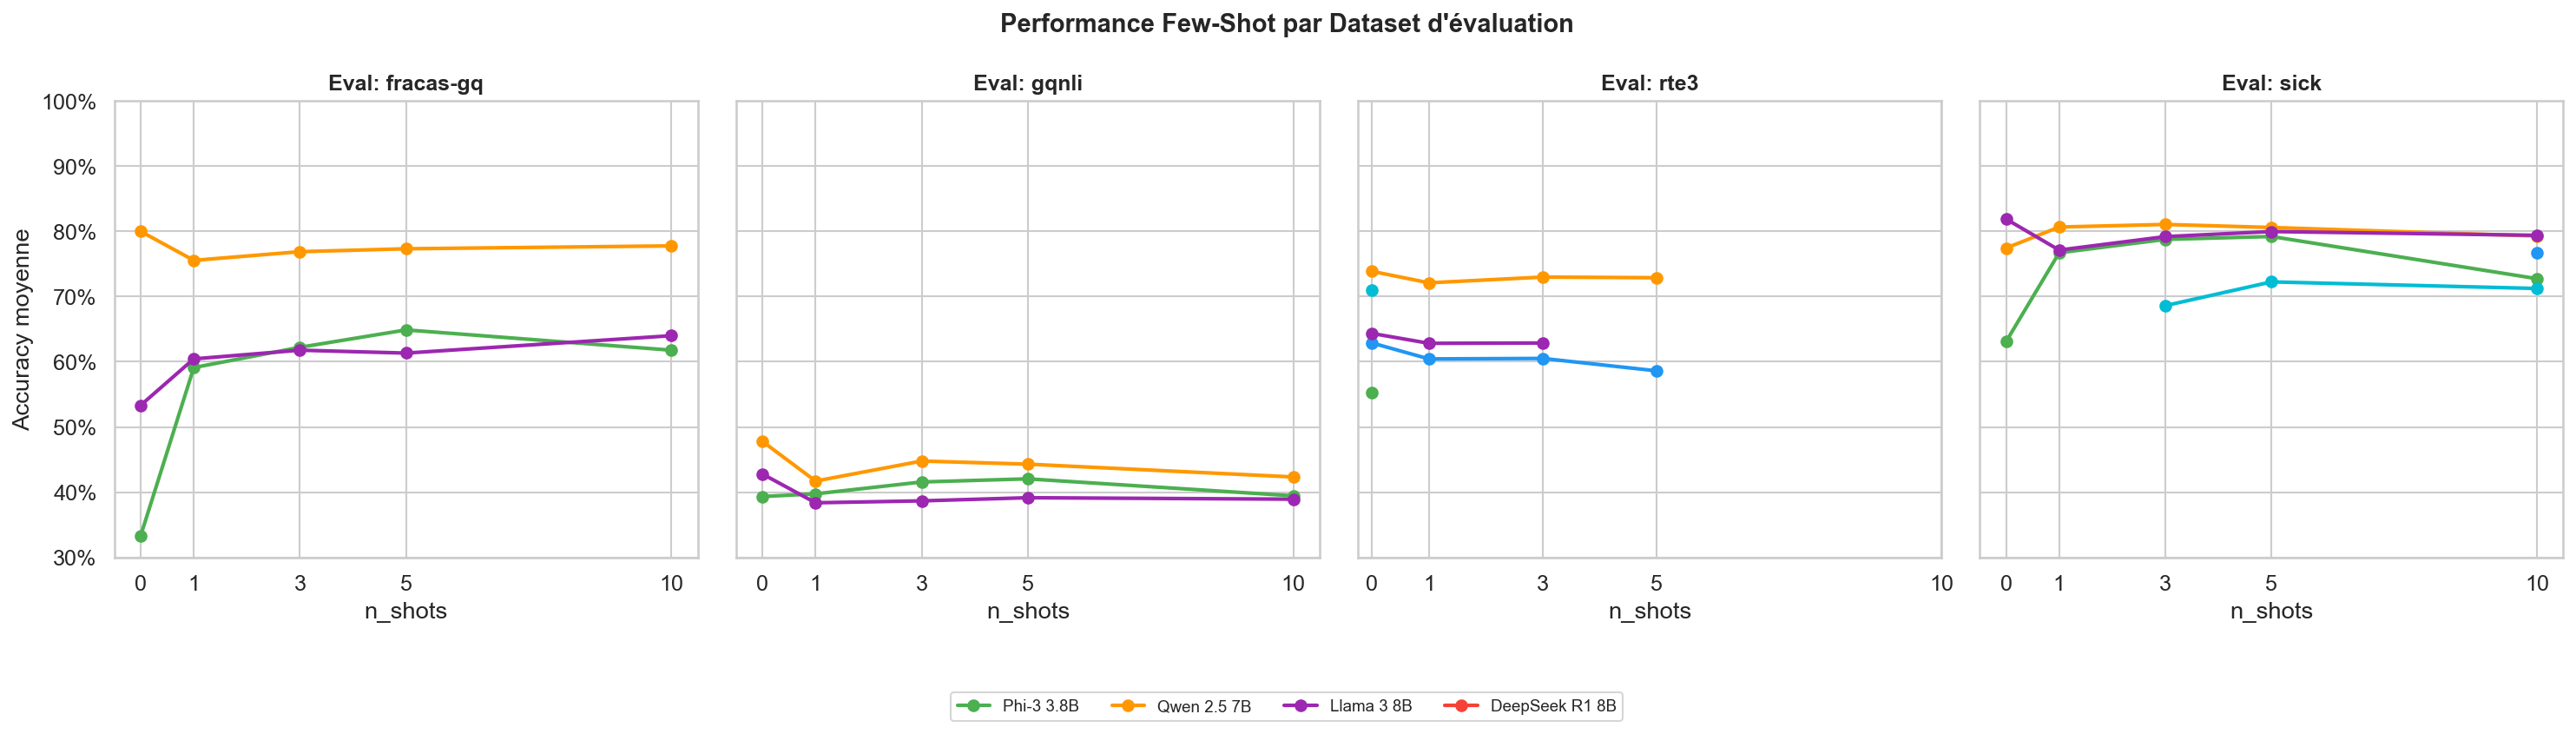
\includegraphics[width=\textwidth]{../results/label_only_plots/fig5_shots_per_eval_dataset.png}
\caption{Évolution de l'accuracy en fonction des shots, séparée par dataset d'évaluation.}
\label{fig:perdataset}
\end{figure}

La Figure~\ref{fig:perdataset} permet de comparer l'effet du few-shot dataset par dataset. On observe que :
\begin{itemize}
    \item Sur \textbf{SICK}, tous les modèles convergent vers des scores élevés (75--80\%) dès quelques shots, quel que soit le dataset source.
    \item Sur \textbf{GQNLI}, les scores restent faibles ($< 50\%$) pour tous les modèles, confirmant la difficulté intrinsèque de ce corpus pour le few-shot label-only.
    \item Sur \textbf{RTE3} et \textbf{FraCaS-GQ}, le few-shot apporte un gain plus progressif et variable selon le modèle.
\end{itemize}

\subsection{Facteurs pouvant influencer les résultats}

Plusieurs facteurs expérimentaux peuvent biaiser ou limiter l'interprétation des résultats :

\paragraph{Déséquilibre du nombre de classes.}
Les datasets RTE3 et DACCORD sont binaires (2 classes), tandis que FraCaS-GQ, GQNLI et SICK sont ternaires (3 classes). La conversion de labels lors des transferts cross-dataset (par ex. \textit{neutral} $\to$ \textit{non-contradiction}) introduit une perte d'information et peut pénaliser artificiellement certaines combinaisons.

\paragraph{Taille de l'ensemble d'évaluation.}
Par contrainte de ressources, l'évaluation est limitée à \textbf{300 exemples} par run, sélectionnés de manière équilibrée par classe. Sur des datasets de petite taille (FraCaS-GQ $\approx$ 330 exemples), cela revient à presque tout le corpus, avec peu de variabilité entre les seeds.

\paragraph{Quantification 4-bit.}
Le chargement en NF4 4-bit réduit l'empreinte mémoire mais peut légèrement dégrader les performances par rapport au modèle en précision complète (bf16/fp16). Cet impact est estimé à 1--3\% d'accuracy selon les études de référence.

\paragraph{Température de génération.}
Tous les modèles sont évalués en mode déterministe (\texttt{do\_sample=False}, greedy decoding). Ce choix garantit la reproductibilité mais peut ne pas refléter les performances optimales du modèle, certains bénéficiant d'un léger échantillonnage pour la diversité.

\paragraph{Biais de langue.}
La tâche est formulée en français, mais certains modèles (notamment Llama 3) ont été entraînés principalement sur de l'anglais. Le système prompt et les exemples sont en français, ce qui peut avantager des modèles mieux alignés pour les langues romanes (Qwen, Gemma, Mistral).

\paragraph{Sélection des exemples few-shot.}
Les exemples sont sélectionnés aléatoirement (avec seed fixée) de façon équilibrée par classe. La qualité des exemples sélectionnés peut varier : un exemple ambigu ou difficile inclus dans le prompt peut dégrader la performance sur tout un batch. L'utilisation de 3 seeds différentes permet d'estimer cette variance.

\subsection{Analyse du plateau de performance}

\subsubsection{Observation : saturation rapide avec les shots}

L'une des observations les plus marquantes est la \textbf{faible croissance des performances} lorsque le nombre de shots augmente. Le Tableau~\ref{tab:plateau} résume l'accuracy moyenne tous modèles confondus :

\begin{table}[h]
\centering
\caption{Accuracy moyenne globale en fonction du nombre de shots.}
\label{tab:plateau}
\begin{tabular}{rcc}
\toprule
\textbf{n\_shots} & \textbf{Accuracy moy.} & \textbf{Gain vs. 0-shot} \\
\midrule
0  & 60.4\% & ---      \\
1  & 62.1\% & +1.7 pts \\
3  & 63.5\% & +3.1 pts \\
5  & 64.4\% & +4.0 pts \\
10 & 63.3\% & +2.9 pts \\
\bottomrule
\end{tabular}
\end{table}

Le gain maximal entre zero-shot et 5-shot n'est que de \textbf{+4 points}, et la courbe s'inverse légèrement à 10 shots. Ce phénomène de \textit{saturation du few-shot} est cohérent avec la littérature récente sur les LLMs.

\subsubsection{Causes identifiées}

\paragraph{1. Dilution par classe.}
La sélection des shots est équilibrée par classe. Avec $k=5$ et 3 classes, seul $\lfloor 5/3 \rfloor = 1$ exemple est fourni par classe. Il faut $k=15$ pour atteindre 5 exemples par classe, seuil jugé nécessaire pour un apprentissage en contexte réellement informatif :

\begin{center}
\begin{tabular}{rcc}
\toprule
\textbf{n\_shots} & \textbf{Ex./classe (3-cls)} & \textbf{Ex./classe (2-cls)} \\
\midrule
5  & 1 & 2  \\
10 & 3 & 5  \\
15 & 5 & 7  \\
20 & 6 & 10 \\
\bottomrule
\end{tabular}
\end{center}

\paragraph{2. Saturation du contexte (Phi-3).}
Phi-3 Mini dispose d'une fenêtre de contexte de \textbf{4 096 tokens}. Avec $\sim$70 tokens par exemple NLI, 10 shots consomment déjà $\sim$700 tokens auxquels s'ajoutent le prompt système ($\sim$150 tokens) et l'exemple test. À 15--20 shots, la contrainte de contexte devient active et peut forcer le modèle à tronquer les premiers exemples.

\paragraph{3. Transfert négatif sur GQNLI.}
GQNLI est le seul dataset pour lequel l'accuracy \textbf{baisse} avec les shots ($-3.1$ pts entre 0 et 10 shots). Ce dataset, centré sur des questions générales ouvertes, présente des paires dont la relation logique est sémantiquement ambiguë. Les exemples few-shot peuvent \textbf{désorienter} le modèle en lui présentant des structures non généralisables, phénomène connu sous le nom de \textit{negative transfer} en in-context learning.

\paragraph{4. Parse rate dégradé de Gemma en zero-shot.}
Gemma 2 9B affiche un parse rate de seulement \textbf{51.6\%} en zero-shot (contre 100\% à 3+ shots). Sans exemples, Gemma génère des réponses longues avec justification, ignorées par le parser. Son score zero-shot est donc calculé sur seulement la moitié des exemples, et potentiellement biaisé. Le few-shot agit ici comme \textbf{signal de format} plutôt que comme aide au raisonnement.

\paragraph{5. Connaissances NLI déjà internalisées.}
Les grands LLMs (Qwen, Gemma, Mistral) ont été pré-entraînés sur des corpus massifs incluant des textes de raisonnement logique. Leur représentation interne de l'implication textuelle est suffisamment développée pour être activée sans exemples. Les shots additionnels n'apportent alors pas d'information nouvelle, voire créent du \textbf{bruit} si les exemples sont atypiques.

\subsubsection{Extension : 15-shot et 20-shot}

Pour investiguer si le plateau peut être dépassé, le sweep a été étendu aux configurations \textbf{15-shot} et \textbf{20-shot}. L'hypothèse est que passer à 5+ exemples par classe (atteint à $k \geq 15$ pour 3 classes) pourrait franchir un seuil d'apprentissage en contexte, en particulier pour Phi-3 et Llama 3 qui ont montré les gains les plus importants.

Deux scénarios sont envisagés :
\begin{itemize}
    \item \textbf{H1 (continuation)} : le gain continue modestement sur SICK et RTE3, où les exemples sont clairement séparables.
    \item \textbf{H2 (dégradation)} : la saturation de contexte (Phi-3) et la redondance informationnelle entraînent une légère baisse, observable surtout sur GQNLI.
\end{itemize}

Les résultats de ces nouvelles configurations seront intégrés à l'issue des sweeps en cours.

\subsection{Conclusion}

Ces expériences démontrent la viabilité de l'approche \textbf{Few-Shot Label-Only} pour la tâche NLI en français sans aucun entraînement. Les performances atteignent jusqu'à \textbf{71.4\%} d'accuracy pour Gemma 2 9B, avec un parse rate de 100\% confirmant que les LLMs modernes respectent les contraintes de format du prompt.

Les principaux enseignements sont :
\begin{enumerate}
    \item L'\textbf{alignement multilingue} prédomine sur la taille en paramètres.
    \item Le \textbf{few-shot bénéficie davantage aux petits modèles} (Phi-3 : +16 pts en zero-to-5-shot).
    \item La \textbf{généralisation cross-dataset} est robuste (écart $< 10\%$).
    \item \textbf{GQNLI reste un verrou} : transfert négatif observé dès 5 shots.
    \item La \textbf{saturation du few-shot} est rapide (plateau à 5 shots), expliquée par la dilution des classes, les connaissances déjà internalisées, et les contraintes de fenêtre de contexte.
\end{enumerate}

% ─────────────────────────────────────────────────────────────────

\end{document}
